\section{Theoretische Grundlagen}

    \subsection{Geschichtliche Hintergründe}

        \noindent 1914 wurde mit dem Franck-Hertz-Versuch mit das erste Mal die Quantennatur der Elektronenhülle von Atomen gezeigt. Es wurde ein 
        Zusammenhang zwischen den Anregungsenergien $\symup{E_a}$ von Hg-Atomen und der Wellenlänge des emmitierten Lichtes bei der Rückkehr 
        in den Grundzustand hergestellt. Somit die von Niels Bohr aufgestellten Bohrschen Postulate über die Natur der Elektronenhülle 
        bestätigt. 

    \subsection{Einleitung und Zielsetzung}

        \noindent Atomhüllen können entweder mithilfe der Atomspektroskopie oder mit Elektronenstoßexperimenten untersucht werden, im Bereich der 
        Atomspektroskopie werden Atome hauptsächlich durch Wechselwirkungen mit elektromagnetischer Strahlung analysiert.\\
        \noindent In diesem Versuch werden jedoch Hg-Atome mit Elektronenstoßexperimenten betrachtet. Dazu werden die Atome mit Elektronen 
        beschossen und die Energieverluste der Elektronen betrachtet. Genauer gesagt werden beim Frank-Hertz-Experiment Elektronen mit 
        möglichst gleicher Energie durch einen Hg-Dampf passender Dichte geführt. Aus den Energiedifferenzen der dabei entstehenden elatischen 
        und unelastischen Stöße lassen sich dann die vom Hg-Atom aufgenommenen Energien berechnen. Bei unelastischen Stößen wird die 
        aufgenommene Energie dazu genutzt das Hg-Atom aus dem Ruhezustand in den ersten angereten Zustand anzuheben. Die Energien verhalten sich 
        nach folgender Beziehung:

        \begin{equation*}
            \frac{m_0 \cdot v_{\text{vor}^2}}{2} - \frac{m_0 \cdot v_{\text{nach}^2}}{2} = E_1 - E_0
        \end{equation*}

        \noindent Die Energien der Elektronen können dann über die Gegenfeld Methode bestimmt werden.
        Insgesamt ist also das Ziel des Frank-Hertz-Versuches die Energie $E_1 - E_0$ und somit die Inonisationsenergie von Hg zu bestimmen, 
        so wie etwas über die Energieverteilung der verwendeten Elektronen zu erfahren.

    \subsection{Der Aufbau und Ablauf}

        \noindent Der Versuch besteht wie in Abbildung(\ref{img:aufb}) zu sehen ist aus einem evakuierten Gefäß, in dem ein Tropfen Quecksilber 
        nach den Verlauf der Dampfdruck-Kurve verdampft. Der Gleichgewichtsdampfdruck $p_\text{sät}$ hängt alser von der Umgebungstemperatur $T$ ab.
        Innerhalb des Glaskolben wird ein hochschmelzendes Metall wie zum Beispiel Wolfram durch einen Gleichstrom bis auf Rotglut erhitzt.
        
        \begin{figure}[ht]
            \centering
            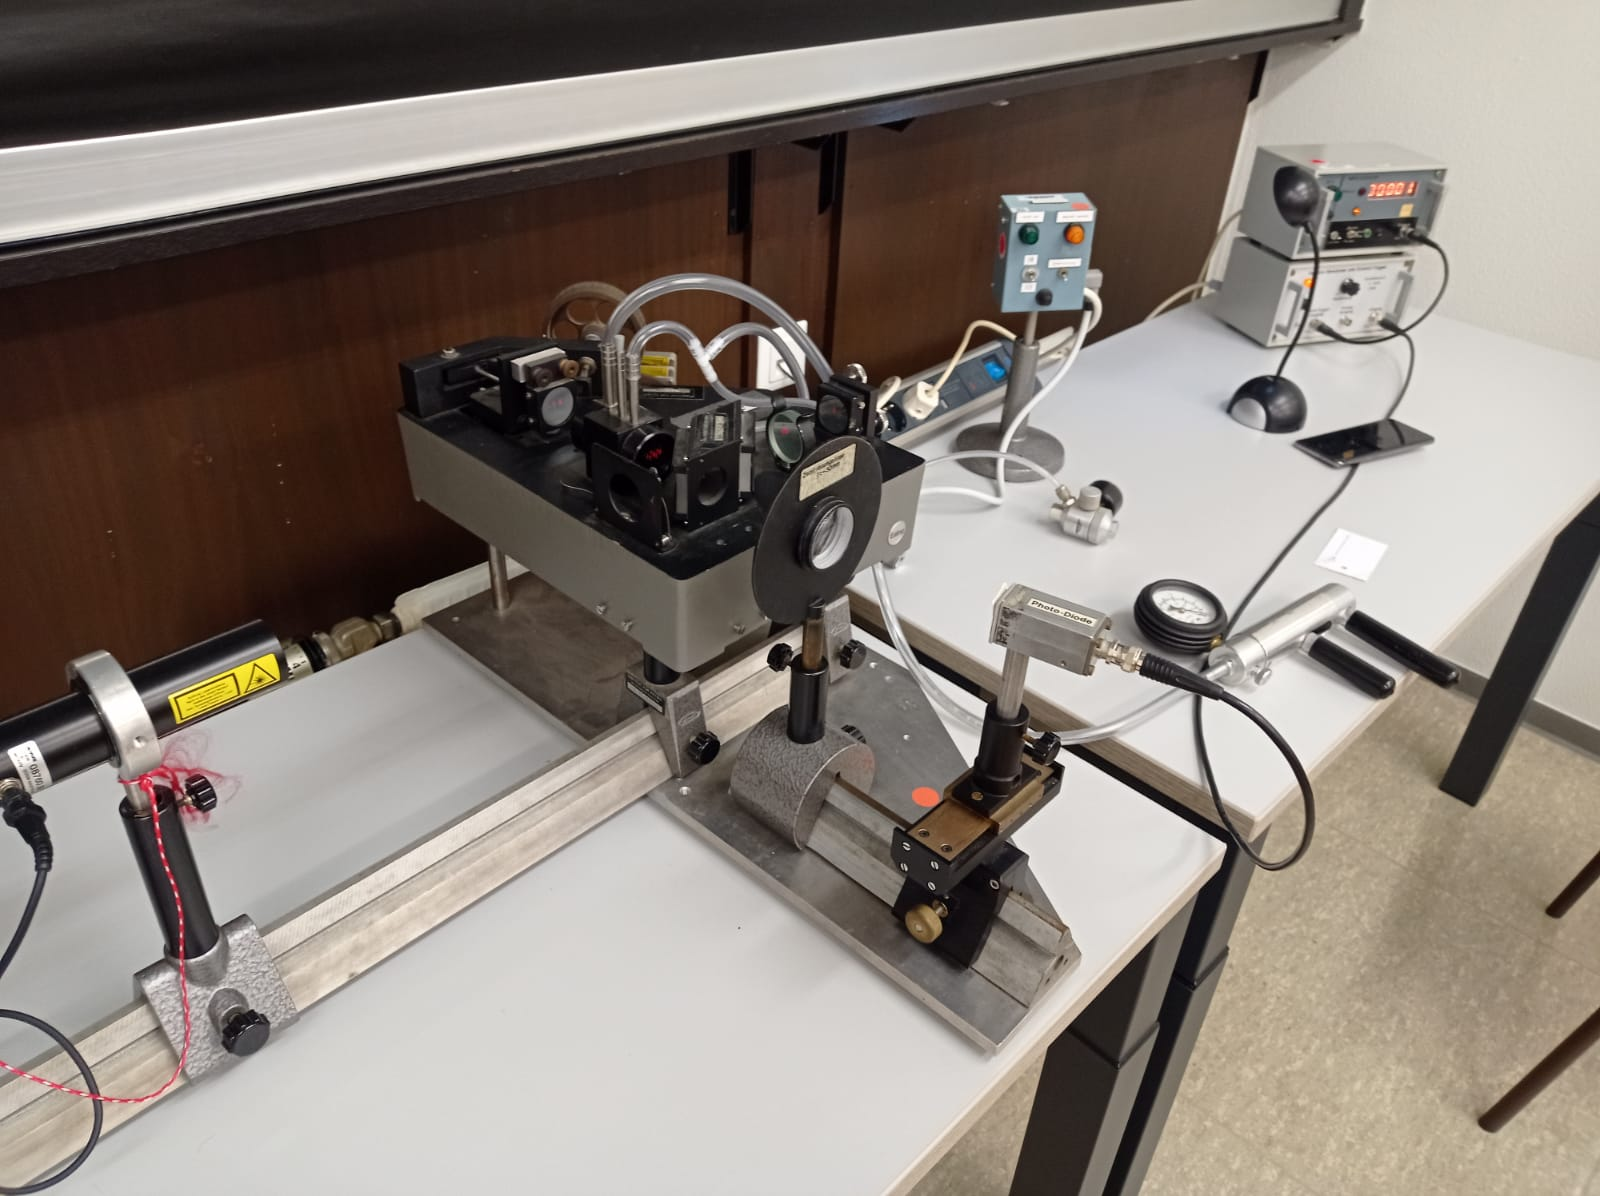
\includegraphics[width=0.7\textwidth]{build/plots/Aufbau.png}
            \caption{Schematischer Aufbau des Frank-Hertz-Versuches.}
            \label{img:aufb}
        \end{figure}

        \noindent Aufgrund des glühelektrischen Effekts treten nun Elektronen aus dem Draht aus, dieser Effekt wird dadurch verstärkt, dass ein 
        Oxid eines Erdalkalimetalles mit einer geringeren Austrittsarbeit auf den Draht aufgetragen wird. Zur Beschleunigung der Elektronen ist 
        gegenüber von dem Glühdraht eine netzförmige Elektrode mit einer positiven Gleichspannung $U_\text{B}$ welche die Elektronen auf eine 
        kinetische Energie des Betrags

        \begin{equation*}
            \frac{m_0 \cdot v_{\text{vor}}^2}{2} = \text{e}_0 U_\text{B}
        \end{equation*}

        \noindent beschleunigt. Bei der Formel wird jedoch nicht berücksichtigt, dass die Elektronen bereits eine Grundenergie besitzen können.
        



        
